\section{Introduction}
Humans handle complex, long-horizon work via collective intelligence and the ability to coordinate~\cite{gao2025evolvesurvey,DBLP:journals/corr/abs-2510-23587,DBLP:journals/corr/abs-2510-17586}. As today's agents are pushed toward similarly complex and multi-turn tasks~\cite{yao2024tau, zhang2025autoenv, xu2026unlocking}, a well-designed agentic system becomes a vital way to scale performance beyond a single model~\cite{liu2025advances}.

\begin{figure}[t!]
    \centering
    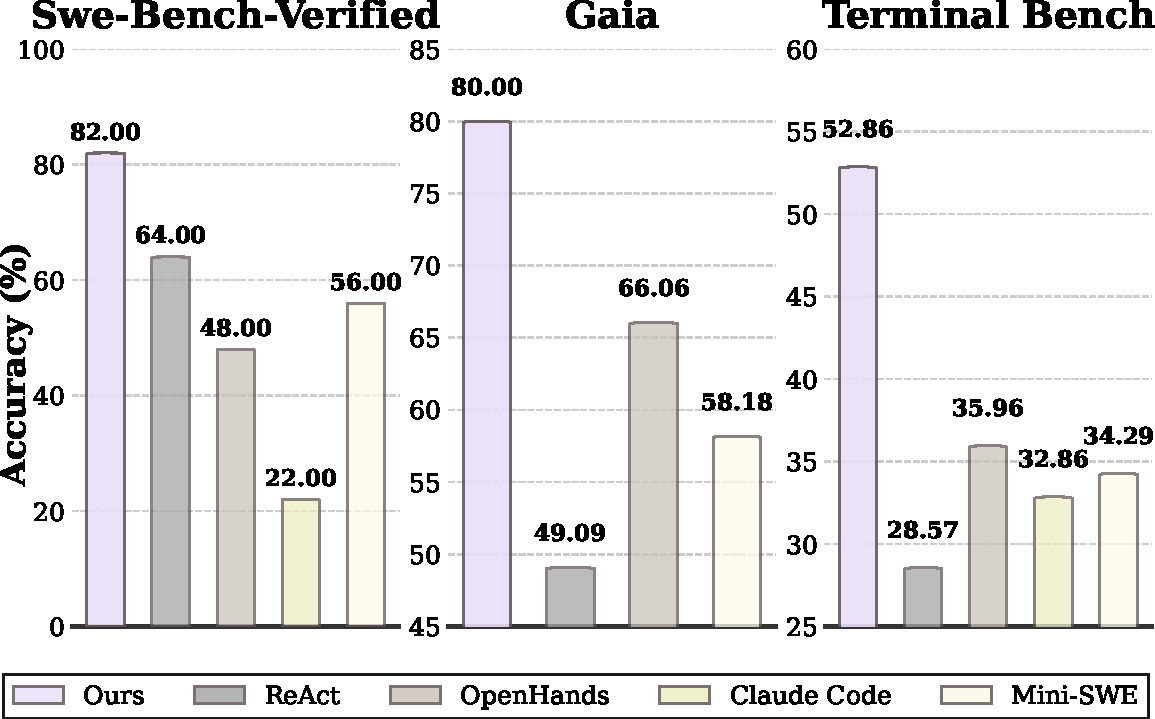
\includegraphics[width=\linewidth]{figures/abs.pdf}
    \caption{Overall performance on three challenging agentic benchmarks (GAIA, Terminal-Bench-2, SWE-Bench-Verified) paired with Gemini-3-Flash when comparing \our against other popular agentic frameworks.}
    \label{fig:performance}
\end{figure}

To cope with increasingly complex scenarios, early attempts rely on fixed coordination workflows or multi-agent systems~\cite{hong2023metagpt, hu2025owl, DBLP:journals/corr/abs-2510-17586}. 
While multi-agent collaboration can improve task decomposition, in open-ended environments it often incurs substantial coordination overhead and provides limited control over context routing, leading to either noisy over-sharing or harmful omission of critical information, which makes robust long-horizon execution difficult~\cite{gao2025single}.

\begin{figure*}[htbp]
    \centering
    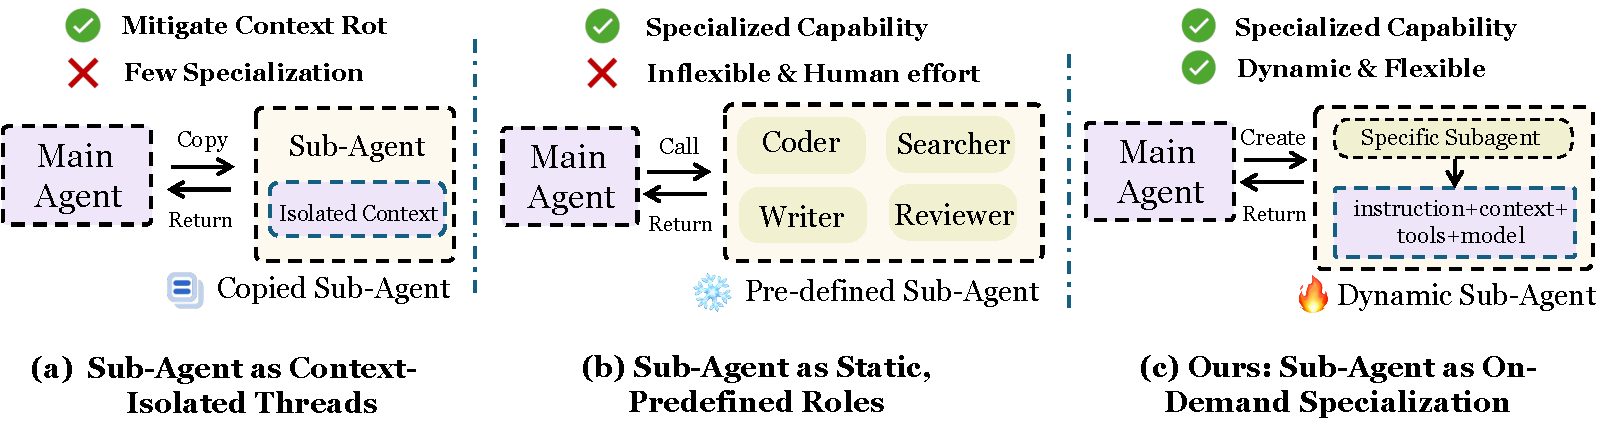
\includegraphics[width=\linewidth]{figures/diff.pdf}
    \caption{Comparison of sub-agent-as-tools approaches. \textbf{(a) Sub-agents as context-isolated threads} mitigate context rot but lack on-demand specialization. \textbf{(b) Sub-agents as static roles} provide specialized capabilities but are inflexible, leave coverage gaps, and require heavy human engineering. \textbf{(c) Our Sub-agents as on-demand specialization} concretizes a unified 4-tuple abstraction \textsc{(Instruction, Context, Tools, Model)} to enable creating tailored executors on the fly.}
    \label{fig:diff}
\end{figure*}

More recent approaches therefore move toward a more practical sub-agent-as-tools paradigm, where a main agent (orchestrator) delegates a task to a sub-agent via an explicit tool call. 
Yet existing designs still lack flexibility in practice and often degenerate into two limited patterns, which are shown in Figure~\ref{fig:diff}:
(1) \textit{Sub-agents as context-isolation threads.} Systems such as ~\citet{schroeder2025thread, sun2025scaling} primarily treat sub-agents as isolated context threads, aiming to prevent context rot~\citep{hong2025context}. However, in real-world tasks, subtasks often require specialized capabilities. Therefore, such systems fail to fully realize the potential of specialized sub-agents. (2) \textit{Sub-agents as static roles.} 
Systems such as ~\citet{anthropic_claude_code_subagents, li2025chain} treat each sub-agent as a static role, and their capabilities or their coordination patterns are typically hard‑wired. A pre-defined set of sub‑agents cannot cover the dynamically emerging variety of subtasks in open environments. Besides, it relies on heavy human engineering, making the system difficult to adapt to various environments.

In this paper, we introduce \our{}, an agentic framework designed to tackle long-horizon and complex tasks. Our core insight lies in treating sub-agents through the lens of \textbf{on-demand specialization}, as illustrated in Figure~\ref{fig:diff}(c). 
We posit that a sub-agent should be viewed as a flexible abstraction unit rather than a predefined, fixed role. This approach enables the system to instantiate tailored sub-agents at runtime by dynamically composing their capabilities to meet specific task demands—an essential feature.
Concretely, \emph{any} agent can be described as an instantiable unit via a unified four-tuple: \textsc{(instruction, context, tools, model)}. This specialization is organized around two complementary axes essential for an agent's task solving: (1) \emph{Working memory (instruction, context):} what the agent must achieve and what evidence it should condition on. Notably, the context attribute is designed to inject only the most relevant information for the current sub-task, filtering out potentially distracting details. (2) \emph{Capabilities (tools, model):} what the agent is empowered to do to accomplish that objective. By composing specific tools and models on a per-subtask basis, we endow each sub-agent with precise, task-specific functionality. Together, this 4-tuple design enables an automatic specialized sub-agent for each task.

Building on this on-demand specialization view, we further introduce a dedicated orchestrator that operates directly over the four-tuple interface to automatically create tailored sub-agents on the fly. It does not execute any tasks and focuses exclusively on orchestration, where we define it as dynamically decomposing the overall objective into the next subtask, creating and delegating a specialized tailored sub-agent for task execution via explicit tool calls.
This decoupling design offers several key advantages. 
First, this dynamic creation allows each sub-agent to be customized with unique capabilities and a clean working context, significantly improving task execution accuracy. 
Second, the orchestrator remains agnostic to the internal implementation of sub-agents, making them fully pluggable. 
Third, the orchestrator can be trained or learned from interactive experience.  
This ranges from basic skills for agent creation to advanced features like adaptive model selection, achieving an optimal balance between cost and performance.

Through extensive experiments, we demonstrate \our{} achieves stronger performance and broader generalization in open‑world settings.
We first evaluate our framework in a training-free setting on three challenging agentic benchmarks: Terminal-Bench 2.0~\cite{tbench_2025} (bash environment), SWE-Bench~\cite{jimenez2023swe} (coding environment), and GAIA~\cite{mialon2023gaia} (digital world environment). As shown in Figure~\ref{fig:performance}, our method consistently outperforms both representative sub-agent orchestration approaches ~\cite{anthropic_claude_code_subagents} and widely used agent frameworks~\cite{wang2024openhands, yang2024sweagent} across all benchmarks. In particular, our framework achieves a 16.28\% improvement when paired with \texttt{Gemini3-Flash}, validating the superiority of our orchestration model in complex, long-horizon tasks. 
% 
Importantly, \our naturally supports learning the orchestration policy from experience.
We instantiate this in two ways: (1) we apply supervised fine-tuning to improve the Orchestrator's subtask decomposition and 4-tuple synthesis, leading to better orchestration quality by +11.51\% pass@1 on GAIA and
(2) we leverage in-context learning to optimize cost-aware routing, which improves GAIA pass@1 by +3.03\% while reducing average cost by 18.5\%, resulting in a more favorable cost--performance Pareto frontier.

Overall, our contributions are:
\begin{itemize}
    \item We propose \our, an orchestrator-centric agentic system that treats sub-agents as \emph{dynamically creatable} executors via a unified 4-tuple interface \textsc{(Instruction, Context, Tools, Model)}, enabling on-demand specialization with task-sufficient context and explicit capability control.
    \item \our achieves strong training-free performance on Terminal-Bench 2.0, SWE-Bench-Verified, and GAIA, consistently outperforming popular agentic systems. We achieve 16.28\% relative improvement against the strongest baseline when paired with Gemini-3-Flash.  
    \item We show the orchestration policy is learnable under this design from two complementary angles: supervised fine-tuning improves basic task orchestration (+11.51\%), and cost-aware routing via in-context learning yields favorable cost--performance Pareto trade-offs (reducing average cost by 18.5\%).
\end{itemize}

